\section{Agentic Video, Film, and Animation Generation}
\label{sec:video-animation}

Video generation extends both the planning horizon and the scope of each correction. Systems work with scripts, shots, keyframes, motion, audio, camera state, and timelines. Even a local edit may disrupt identity or causality several shots later. We therefore distinguish staged pipelines from systems that carry temporal state forward, locate failures, and revise the affected material. Figure~\ref{fig:ch5-video-overview} summarizes these mechanisms across the video-production lifecycle.

\begin{figure}[t]
  \centering
  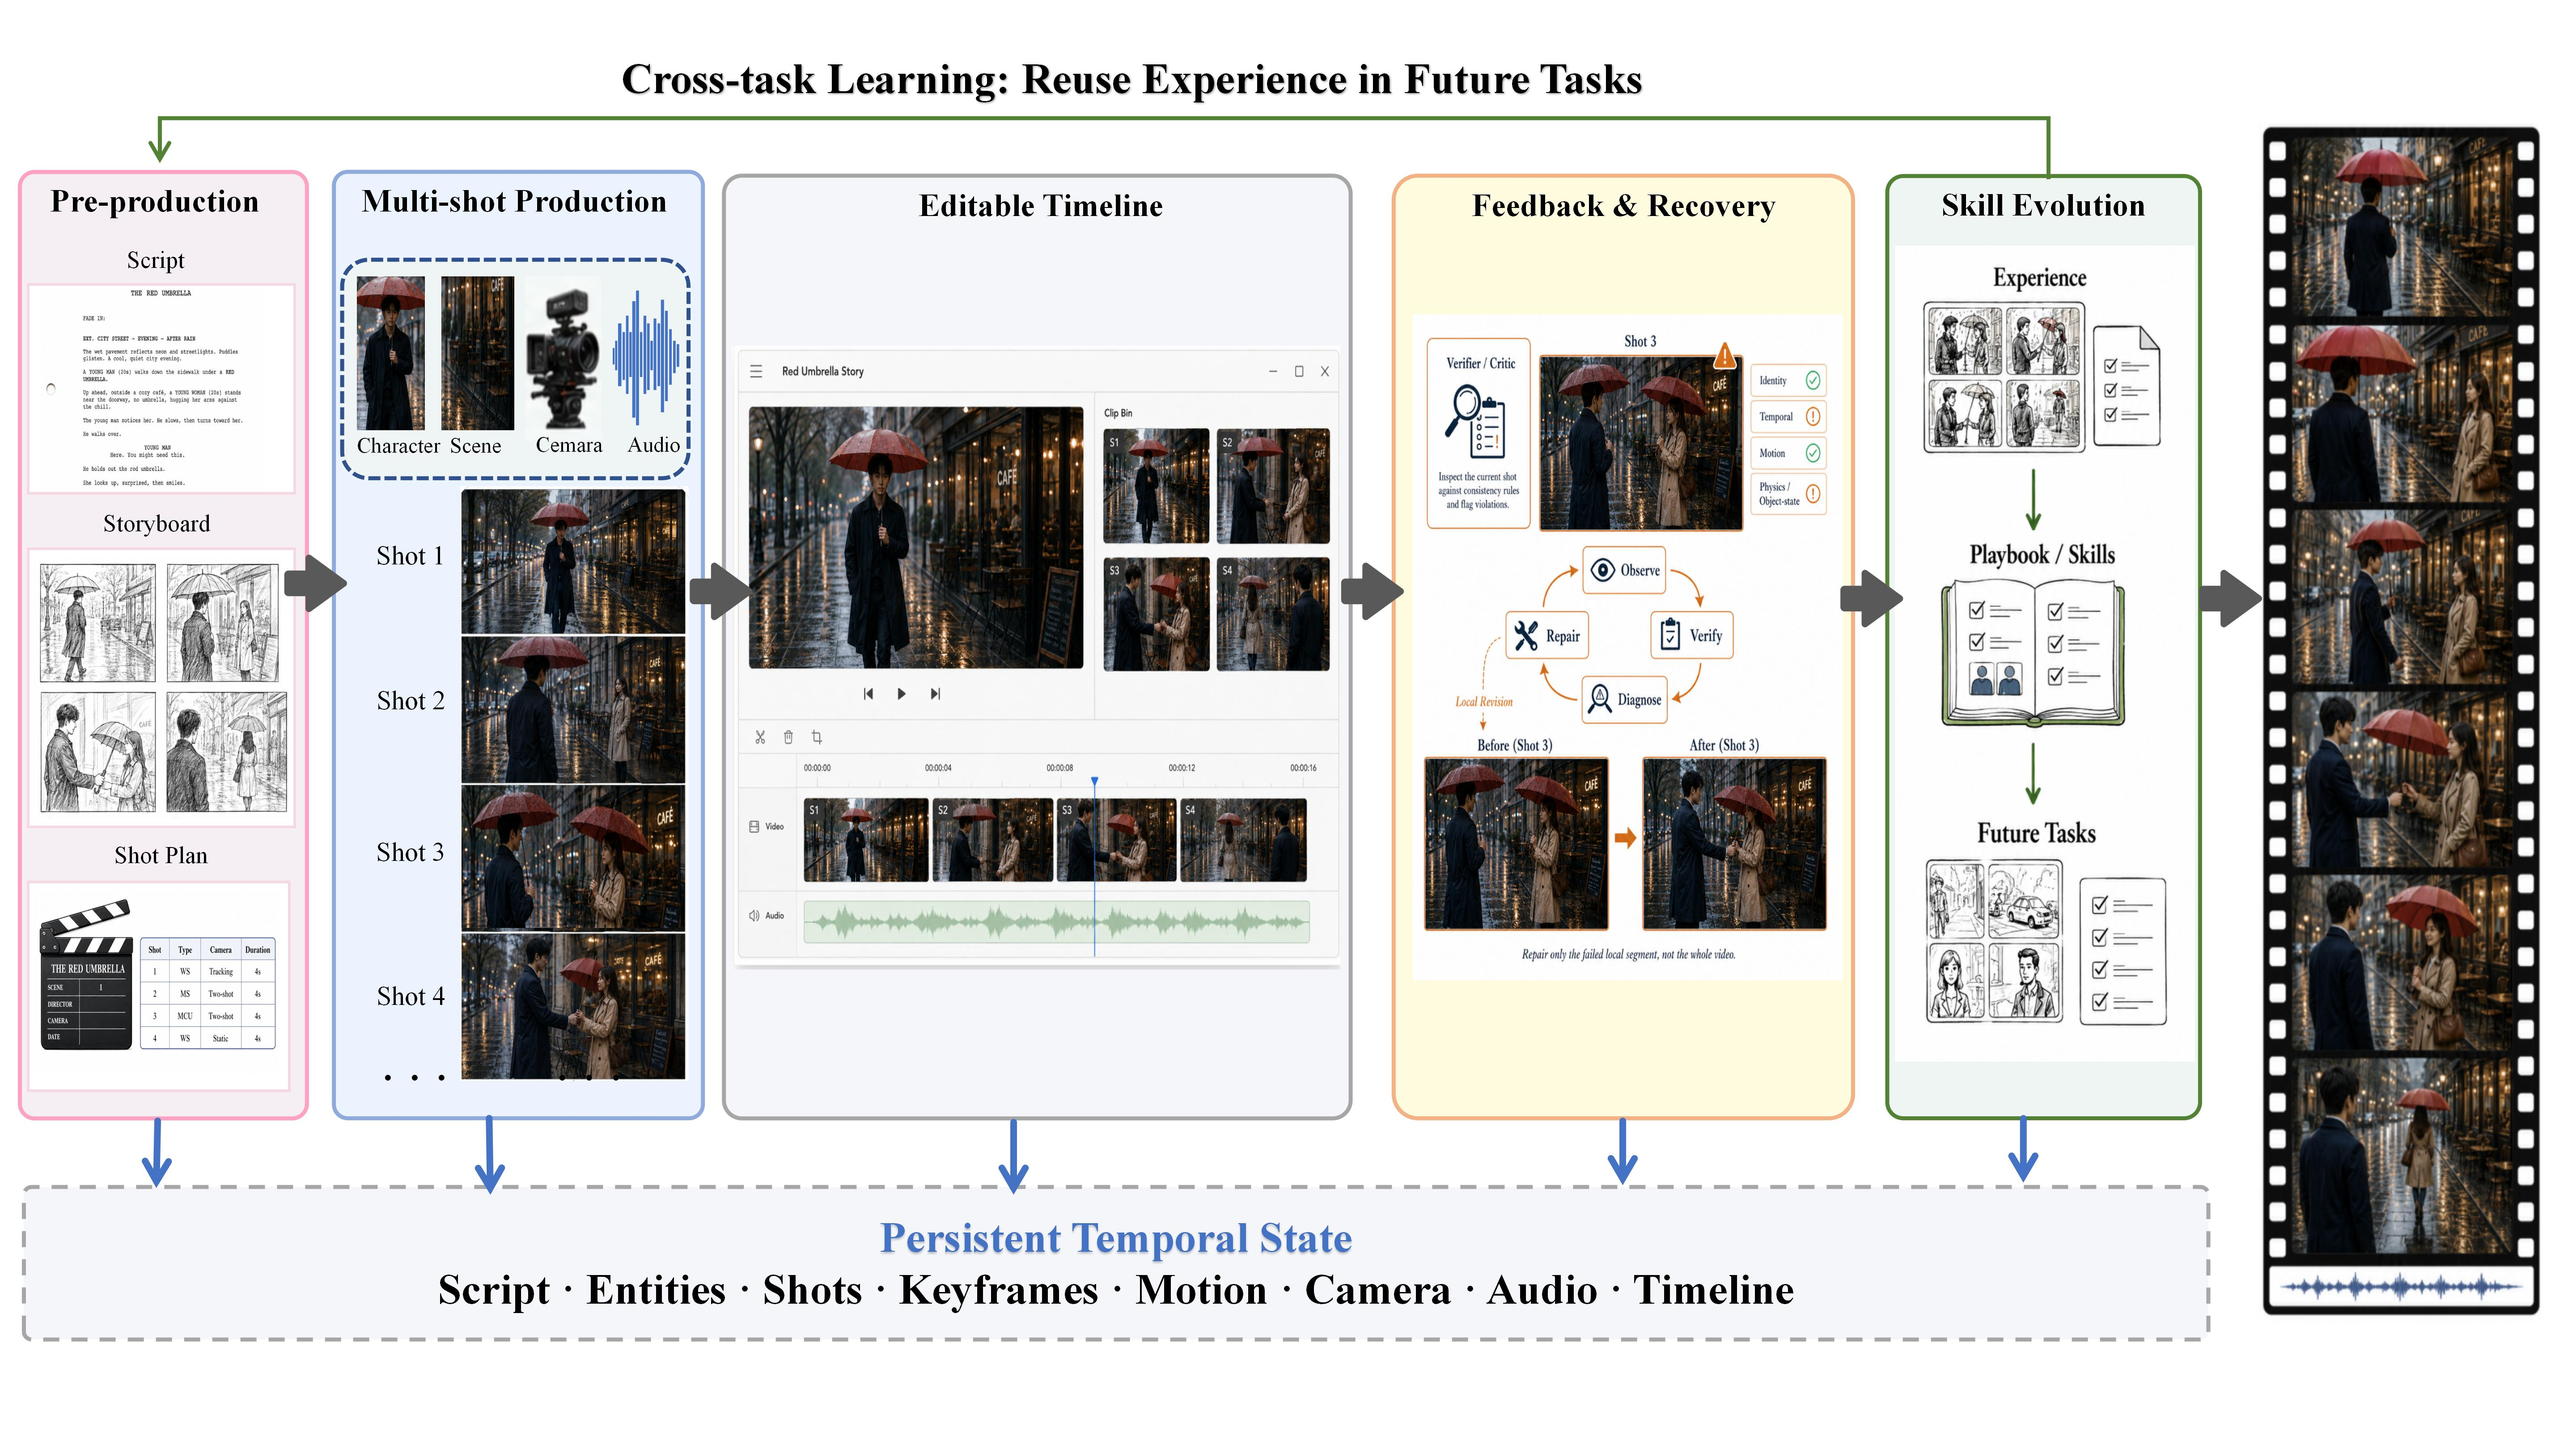
\includegraphics[width=\textwidth]{figures/ch5_agentic_video_generation_overview.jpg}
  \caption{Overview of agentic video generation across the production lifecycle. Pre-production representations guide multi-shot generation and timeline editing; feedback and recovery revise failed local segments, while a persistent temporal state carries scripts, entities, shots, keyframes, motion, camera, audio, and timeline information across stages. Verified experience can further be abstracted into reusable skills for future tasks.}
  \label{fig:ch5-video-overview}
\end{figure}

\begin{keytakeaway}[Agentic Video Generation at a Glance]
\begin{keypoints}
  \item \textbf{Scripts, storyboards, motion, and pre-production:} turn long-range intent into scripts, shot plans, storyboards, trajectories, or motion programs, while preserving the specified characters, settings, and constraints.

  \item \textbf{Multi-shot production and cross-modal orchestration:} assign directing, cinematography, character and scene management, audio, and generation to different agents, with the main distinction being what information passes between them and whether observed results can change later decisions.

  \item \textbf{Editable timelines and post-production:} map language to precise temporal spans, preserve untouched material, and retain enough production history to make later revisions traceable.

  \item \textbf{Temporal feedback, physical control, and local recovery:} identify the failed interval and its likely cause, then repair individual shots, prompts, trajectories, or code instead of regenerating the full sequence.

  \item \textbf{Skill evolution and diagnostic evidence:} go beyond one-off correction by retaining what previous failures reveal and converting diagnostic evidence into reusable prompting strategies or composition skills.
\end{keypoints}
\end{keytakeaway}

\begin{figure}[!htbp]
  \centering
  
\definecolor{avgmapblue}{HTML}{22558A}
\definecolor{avgmapgreen}{HTML}{23845D}
\ifdefined\avgmapfont\else\newcommand{\avgmapfont}{\rmfamily}\fi
\makebox[\linewidth][c]{%
\resizebox{0.98\linewidth}{!}{%
\begin{tikzpicture}[
  avg branch/.style={draw=avgmapblue!58, fill=avgmapblue!9, text=black!88, rounded corners=2.5pt, line width=0.48pt, text width=42mm, minimum height=8.8mm, align=center, inner xsep=2.2mm, inner ysep=0.9mm, outer sep=0pt, execute at begin node={\hyphenpenalty=10000\exhyphenpenalty=10000\relax}, font=\avgmapfont\fontsize{7.35}{8.35}\selectfont\bfseries},
  avg papers/.style={draw=avgmapblue!25, fill=avgmapblue!2, text=black!88, rounded corners=2.5pt, line width=0.38pt, text width=115mm, minimum height=8.8mm, align=left, inner xsep=3mm, inner ysep=0.9mm, outer sep=0pt, execute at begin node={\hyphenpenalty=10000\exhyphenpenalty=10000\relax}, font=\avgmapfont\fontsize{7.15}{8.25}\selectfont\bfseries},
  avg benchmark branch/.style={avg branch, draw=avgmapgreen!78, fill=avgmapgreen!15, text=avgmapgreen!45!black},
  avg benchmark papers/.style={avg papers, draw=avgmapgreen!72, fill=avgmapgreen!7, text=black!88},
  avg root/.style={draw=avgmapblue, fill=avgmapblue!94!black, text=white, rounded corners=2.5pt, line width=0.55pt, minimum width=9mm, minimum height=36mm, inner sep=0pt, outer sep=0pt},
  avg line/.style={draw=black!28, line width=0.45pt, line cap=round},
  avg benchmark line/.style={draw=avgmapgreen!78, line width=0.55pt, line cap=round}
]
\matrix (avgmap) [matrix of nodes, row sep=1.35mm, column sep=3mm, ampersand replacement=\&, nodes={anchor=center}] {
  \node[avg branch] (c5b1) {Scripts and Pre-production}; \& \node[avg papers] (c5p1) {Anim-Director~\cite{avg240809787}, AnimAgents~\cite{avg251117906}, Mind-of-Director~\cite{avg260314790}, AnimeAgent~\cite{avg260220664}.}; \\
  \node[avg branch] (c5b2) {Multi-shot Orchestration}; \& \node[avg papers] (c5p2) {AniME~\cite{avg250818781}, Cutscene Agent~\cite{avg260425318}, DreamFactory~\cite{xie2024dreamfactory}, Google Flow~\cite{roman2026flowagents}, FilmWorld~\cite{avg260719038}.}; \\
  \node[avg branch] (c5b3) {Timelines and Post-production}; \& \node[avg papers] (c5p3) {LAVE~\cite{wang2024lave}, EditDuet~\cite{avg250910761}, Aurora~\cite{avg260518748}, CutClaw~\cite{avg260329664}, DIRECT~\cite{avg260404875}.}; \\
  \node[avg branch] (c5b4) {Feedback and Recovery}; \& \node[avg papers] (c5p4) {VISTA~\cite{long2026vista}, GenMAC~\cite{huang2024genmac}, MoReGen~\cite{avg251204221}, PhysAgent~\cite{li2026physagent}, SCMAPR~\cite{avg260405489}.}; \\
  \node[avg branch] (c5b5) {Skill Evolution and Diagnostics}; \& \node[avg papers] (c5p5) {SCPE~\cite{avg260619073}, VideoWeaver~\cite{avg260608091}.}; \\
  \node[avg benchmark branch] (c5b6) {Benchmarks}; \& \node[avg benchmark papers] (c5p6) {CutsceneBench~\cite{avg260425318}.}; \\
};
\coordinate (c5trunktop) at ($(c5b1.west)+(-4.6mm,0)$);
\coordinate (c5trunkbottom) at ($(c5b6.west)+(-4.6mm,0)$);
\coordinate (c5rootnw) at ($(c5b1.north west)+(-15.5mm,0)$);
\coordinate (c5rootse) at ($(c5b6.south west)+(-7.6mm,0)$);
\node[avg root, fit=(c5rootnw)(c5rootse)] (c5root) {};
\node[rotate=90, align=center, text=white, font=\avgmapfont\fontsize{7.05}{8.15}\selectfont] at (c5root.center) {{\bfseries CHAPTER 5}\\[0.55mm]{\fontsize{6.2}{7.15}\selectfont Video, film, and animation}};
\draw[avg line] (c5trunktop) -- (c5trunkbottom);
\coordinate (c5trunkmid) at ($(c5trunktop)!0.5!(c5trunkbottom)$);
\draw[avg line] (c5root.east) -- (c5trunkmid);
\draw[avg line] (c5trunktop |- c5b1.west) -- (c5b1.west);
\draw[avg line] (c5b1.east) -- (c5p1.west);
\draw[avg line] (c5trunktop |- c5b2.west) -- (c5b2.west);
\draw[avg line] (c5b2.east) -- (c5p2.west);
\draw[avg line] (c5trunktop |- c5b3.west) -- (c5b3.west);
\draw[avg line] (c5b3.east) -- (c5p3.west);
\draw[avg line] (c5trunktop |- c5b4.west) -- (c5b4.west);
\draw[avg line] (c5b4.east) -- (c5p4.west);
\draw[avg line] (c5trunktop |- c5b5.west) -- (c5b5.west);
\draw[avg line] (c5b5.east) -- (c5p5.west);
\draw[avg benchmark line] (c5trunktop |- c5b6.west) -- (c5b6.west);
\draw[avg benchmark line] (c5b6.east) -- (c5p6.west);
\end{tikzpicture}%
}%
}

  \caption{Representative systems and benchmarks for agentic video, film, and animation generation, organized according to the chapter taxonomy.}
  \label{fig:ch5-representative-systems}
\end{figure}

\subsection{Scripts, storyboards, motion, and pre-production.}
Pre-production turns long-range intent into scripts, shot plans, storyboards, trajectories, or motion programs. These representations clarify what should happen, but downstream generators must still preserve the specified characters, settings, and constraints.

\paragraph{Anim-Director}
 uses an LMM as an autonomous director to turn a short narrative into a multi-scene animation. It expands the story into a structured script with character, setting, and scene descriptions, generates reference and scene images, and checks their consistency before using the selected images to guide video generation. The LMM also evaluates and selects image and video candidates during generation~\cite{avg240809787}.

\paragraph{Agentic Aerial Cinematography}
 translates a director's free-form language instruction into an executable indoor UAV video tour. It uses vision--language retrieval to select initial waypoints, refines camera poses through preference-based Bayesian optimization with aesthetic feedback, and plans safe, dynamically feasible quadrotor trajectories~\cite{avg250916176}.

\paragraph{AnimAgents}
 supports animation pre-production through dedicated boards for ideation, design, scripting, and storyboarding. A stage-aware Core Agent coordinates specialized agents and carries relevant project context across stages, while creators can select and refine individual elements without regenerating entire outputs~\cite{avg251117906}.

\paragraph{Automated Movie Generation}
MovieAgent uses hierarchical multi-agent planning to turn a script synopsis and character bank into a structured multi-scene, multi-shot movie plan. A Director Agent organizes the narrative, while Scene Plan and Shot Plan agents progressively specify scenes, character interactions, camera movements, shot types, and dialogue before customized video and audio models generate the final shots~\cite{avg250307314}.

\paragraph{Lighting-grounded Video Generation}
LiVER enables controllable video generation by representing scene layout, lighting, and camera trajectory as explicit 3D conditions. A scene agent translates high-level user instructions into an editable 3D scene representation, whose rendered control signals are then used to condition a video diffusion model~\cite{avg260407966}.

\paragraph{The Script is All You Need}
ScripterAgent translates coarse dialogue into a fine-grained, executable cinematic script that provides shot-level guidance for subsequent video generation. DirectorAgent then executes the script through cross-scene continuous generation with frame anchoring, carrying visual context between scenes to improve long-horizon continuity~\cite{avg260117737}.

\paragraph{Mind-of-Director}
As a boundary case, Mind-of-Director produces an editable 3D film previsualization rather than a finished video. From an initial creative idea, specialized agents iteratively develop the script, construct semantically aligned 3D scenes, plan character blocking and motion, and optimize camera framing and movement, while a real-time visual editor allows creators to inspect the result and adjust the synchronized timeline before production~\cite{avg260314790}.

\paragraph{AnimeAgent}
 is an I2V-based multi-agent framework for custom storyboard generation. A Director converts the story and visual references into a structured textual dope sheet, while an Artist generates continuous motion trajectories with an image-to-video model. A Consistency Reviewer detects identity, pose, and layout errors and feeds them back for revision, while a mixed subjective--objective reviewer selects the most expressive frames as the final storyboard~\cite{avg260220664}.
 

\subsection{Multi-shot production and cross-modal orchestration.}
Production systems assign directing, cinematography, character and scene management, audio, and generation to different agents. The main distinction is what information passes between them and whether observed results can change later decisions.

\paragraph{AniMaker}
 is a multi-agent framework for long-form animated storytelling. A Director Agent creates the storyboard, a Photography Agent uses MCTS-Gen to efficiently explore and generate promising clip candidates, and a Reviewer Agent evaluates them with AniEval for story-level consistency, action completion, and animation quality. A Post-Production Agent then assembles the selected clips and adds editing and voiceover~\cite{avg250610540}. Figure~\ref{fig:ch5-planning-production} compares this storyboard-driven production path with editable 3D previsualization.

\begin{figure}[p]
  \centering
  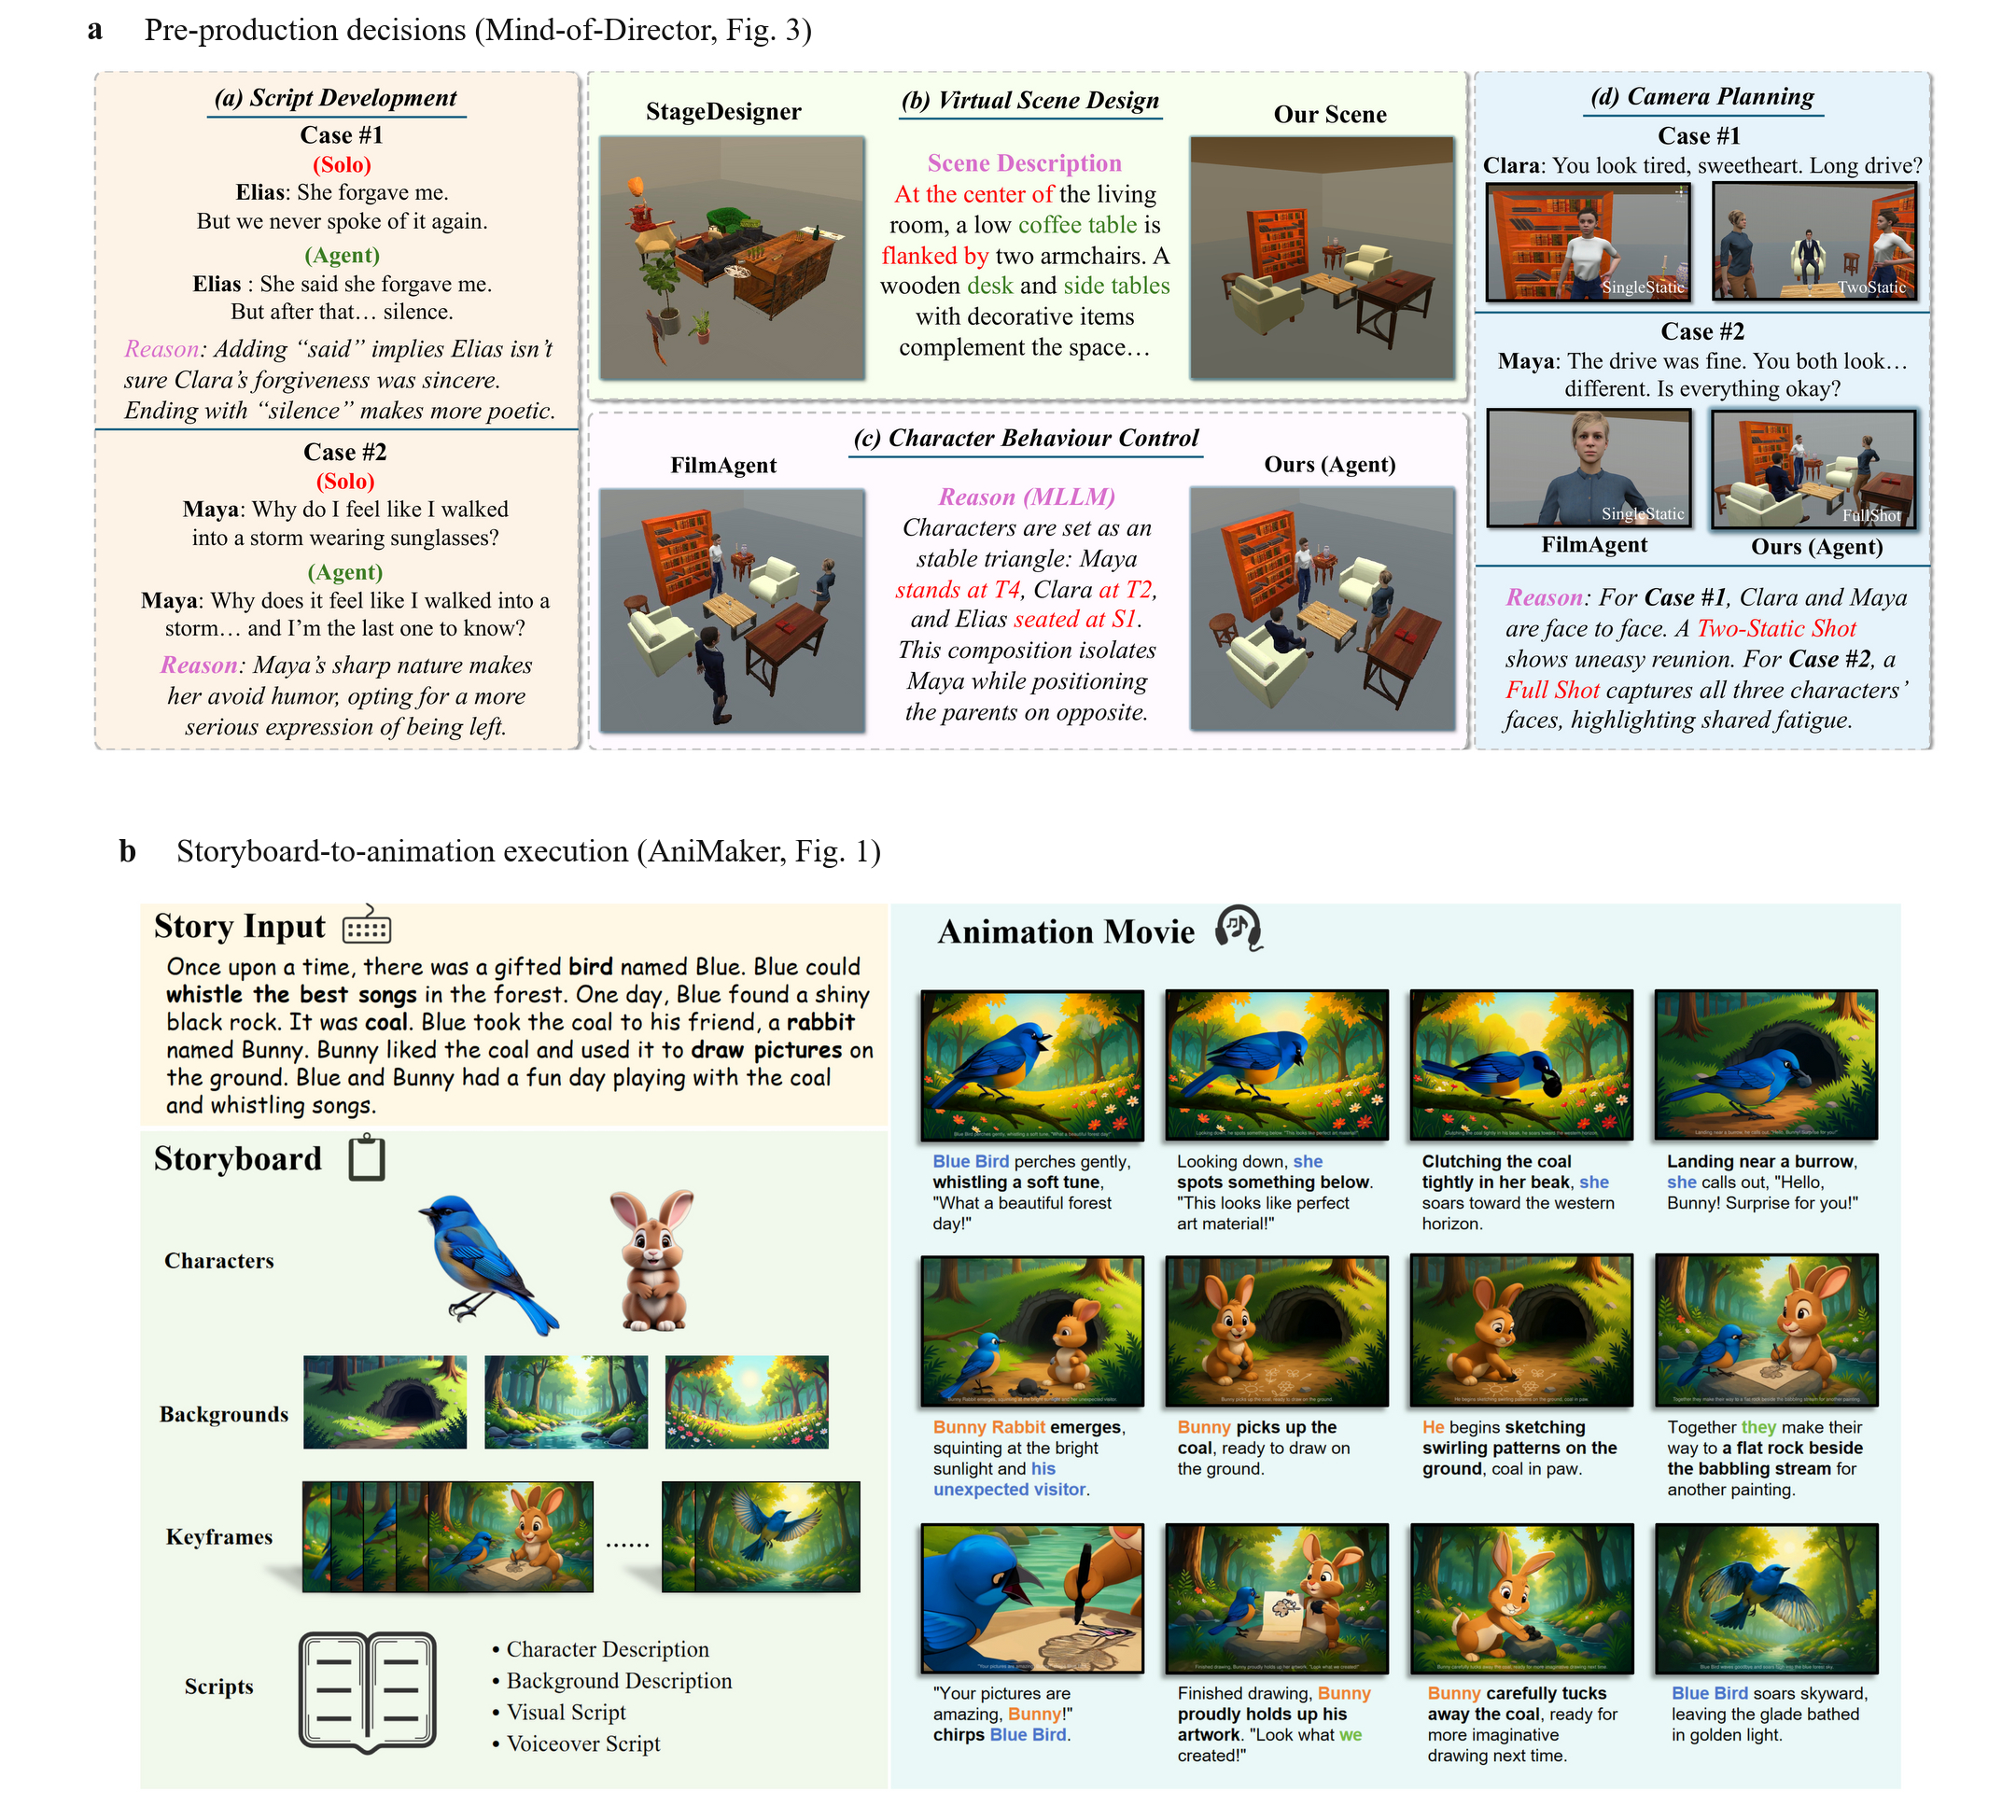
\includegraphics[width=\textwidth]{figures/ch5_planning_production.jpg}
  \caption{Representative pathways from pre-production to multi-shot generation. (a) Mind-of-Director makes script development, virtual scene design, character behavior control, and camera planning explicit in an editable 3D previsualization. (b) AniMaker transforms narrative input into storyboard assets and a multi-scene animation, illustrating how intermediate representations structure long-horizon production~\cite{avg260314790,avg250610540}.}
  \label{fig:ch5-planning-production}
\end{figure}

\paragraph{AniME}
 is a director-oriented multi-agent system for long-form anime production from story to final video. A central Director Agent decomposes the story into dependent production tasks, maintains a shared Asset Memory Bank, and coordinates specialized agents for character and scene design, storyboarding, animation, audio, and editing. Each specialized agent uses an MCP-based toolset to select appropriate models for its task, while quality evaluation can trigger targeted revisions~\cite{avg250818781}.

\paragraph{Cutscene Agent} automates end-to-end 3D cutscene production through an MCP-based Cutscene Toolkit that gives LLM agents bidirectional access to the game engine: agents not only invoke engine operations but continuously observe real-time scene state, enabling closed-loop generation of editable, engine-native cinematic assets~\cite{avg260425318}. A director agent orchestrates specialist subagents for animation, cinematography, and sound design under a visual reasoning feedback loop, and the accompanying CutsceneBench evaluates long-horizon orchestration of dozens of interdependent, strictly ordered tool calls.
 

\paragraph{DreamFactory}
 organizes LLM agents as a virtual film-production team for multi-scene long-video generation. During iterative keyframe creation, a visual Monitor extracts persistent style, background, and character information from generated frames, while contextual information from the current scene is carried into subsequent rounds to guide later keyframes and maintain cross-scene consistency~\cite{xie2024dreamfactory}.

\paragraph{Kubrick}
 generates synthetic videos through collaboration among Director, Programmer, and Reviewer agents. The Director decomposes a text description into filmmaking sub-tasks, the Programmer translates them into Blender Python scripts, and the Reviewer inspects intermediate renders and character motion to provide feedback. The Programmer then iteratively revises the scripts based on this feedback before the final video is rendered~\cite{he2024kubrick}.

\paragraph{Mora}
 is a multi-agent framework that combines specialized open-source modules to support six video-generation tasks, including text-to-video, image-to-video, video extension, editing, video connection, and digital-world simulation. Its agents are jointly adapted through a self-modulation mechanism, while synthetic data generation and human-assisted filtering provide training supervision. At inference time, these modules are largely composed through predefined task workflows rather than an explicit artifact-conditioned feedback loop~\cite{yuan2024mora}.

\paragraph{StoryAgent}
 is a multi-agent framework for generating customized storytelling videos from a narrative and a reference subject. Specialized agents handle story design, storyboard generation, video creation, coordination, and result evaluation, with an Observer providing feedback to the relevant agent when outputs need improvement. A subject-aware storyboard pipeline preserves protagonist identity across shots, while LoRA-BE improves temporal consistency within each shot~\cite{avg241104925}.

\paragraph{AutoMV}
 generates full-length music videos through a music-aware multi-agent pipeline. Music-processing tools extract song structure, vocals, and time-aligned lyrics; a Screenwriter organizes these cues into a shot-level narrative and shared character bank, while a Director prepares keyframes and video instructions for each shot. A Verifier checks generated candidates for script alignment, character consistency, and physical feasibility, allowing weak outputs to be regenerated or replaced before final assembly~\cite{avg251212196}.

\paragraph{Communicative Agents for Slideshow Storytelling}
VGTeam generates slideshow-style narrative videos through a Chat Tower of role-specialized LLM agents. A Director coordinates editor, painter, and composer agents, while shared captions and a Memory Stream carry narrative context across stages. The Director reviews intermediate outputs and returns revision feedback when needed, and image, speech, and music APIs produce the assets assembled into the final video~\cite{avg250901277}.

\paragraph{Hollywood Town}
 introduces OmniAgent, a hierarchical graph-based multi-agent framework for minute-scale video production. Temporary hypergraph discussions allow selected agents to share task-relevant context on demand, while bounded backward connections let downstream agents request revisions from earlier production stages. This enables cross-stage feedback and iterative refinement without requiring every agent to maintain the full production history~\cite{avg251022431}.

\paragraph{MAViS}
 is an end-to-end multi-agent framework for long-sequence video storytelling, coordinating specialized agents for script writing, shot design, character modeling, keyframe generation, animation, and audio generation. At each stage, agents follow an Explore--Examine--Enhance procedure to inspect and refine intermediate results, while dedicated script-writing guidelines adapt the narrative to the capabilities of downstream generative tools~\cite{avg250808487}.

\paragraph{MM-StoryAgent}
 generates narrated storybook videos by coordinating agents across text, image, and audio modalities. A multi-stage writing pipeline first develops the story, after which modality-specific agents iteratively refine prompts for illustrations, narration, music, and sound effects. Character descriptions and consistency-aware image generation help preserve recurring roles, and a composition agent combines the resulting visual and audio assets into the final video~\cite{avg250305242}.

\paragraph{UniVA}
 is an open-source video generalist that unifies video understanding, segmentation, editing, and generation within a Plan-and-Act architecture. A Planner interprets user intent and decomposes it into structured steps, while executor agents invoke modular MCP tools for analysis and video manipulation. Hierarchical memory preserves global knowledge, task context, and user preferences across multi-step interactions, supporting iterative and self-reflective video workflows~\cite{avg251108521}.

\paragraph{Google Flow}
 is an AI creative studio whose Flow Agent plans and reasons through creative tasks using user inputs and project context. It supports brainstorming, generation, editing, parallel variation, and batch revision across project assets, while Gemini Omni allows users to iteratively refine videos through conversation~\cite{roman2026flowagents}.

 \paragraph{Luma Agents}
 is a deployed multimodal creative system that coordinates image, video, audio, and editing models within a shared project workspace. Creative agents maintain project context, route tasks across specialized models, and evaluate generated assets before advancing or revising the production process. The available evidence comes from first-party product documentation rather than an independently evaluated technical study~\cite{luma2026agents}.

\paragraph{Beyond End-to-End Video Models}
LASEV generates educational videos through a hierarchical multi-agent workflow rather than direct end-to-end video synthesis. An Orchestrating Agent coordinates specialized agents for problem solving, executable illustrations, and pedagogical narration, while semantic critiques, rule-based checks, and compilation tests provide iterative quality control. The resulting executable video script is then compiled into synchronized visuals and narration~\cite{avg260211790}.

\paragraph{BrandFusion}
 is a multi-agent framework for integrating advertiser brands into text-to-video generation while preserving user intent and natural scene composition. An offline phase builds a shared Brand Knowledge Base from model priors and adapts the system to novel brands, while five online agents iteratively refine user prompts using this knowledge and real-time contextual tracking to improve brand visibility, recognizability, and semantic alignment~\cite{avg260302816}.

\paragraph{Camera Artist}
 is a multi-agent framework for long-form narrative video generation with explicit cinematic language. Its Cinematography Shot Agent recursively plans each shot from the global script, current scene, and preceding shot to maintain shot-to-shot narrative continuity, then enriches the resulting descriptions with professional cinematic language. A Video Generation Agent uses these shot descriptions together with character and scene references to render and assemble the final video~\cite{avg260409195}.

\paragraph{Co-Director}
 formulates generative video storytelling as hierarchical optimization rather than a fixed chain of prompted modules. A multi-armed bandit explores global creative configurations, while a local multimodal self-refinement loop evaluates generated results and corrects inconsistencies such as identity drift. This combination supports both creative exploration and sequence-level coherence across the resulting narrative~\cite{avg260424842}.

\paragraph{MAVIN}
 generates synchronized multi-shot audio-visual narratives from free-form prompts and optional character references. A lightweight multi-agent scripting pipeline parses shot structure, aligns character identities with visual and audio references, and refines the result into hierarchical global-, shot-, and role-level captions. Boundary-aware attention enforces temporal alignment across shots and dialogue intervals, while ID-aware propagation binds recurring characters to consistent visual appearances and vocal timbres~\cite{avg260629473}.

\paragraph{Sima 1.0}
 organizes long-form documentary production as a hybrid human--agent workflow. Human creators retain core creative decisions and physical recording, while junior and senior AI agents handle labor-intensive tasks such as caption refinement, asset collection, split-level editing, B-roll integration, and final asset preparation. During editing, agents can also source additional materials when visual coverage is insufficient, introducing limited runtime adaptation into an otherwise structured production pipeline~\cite{avg260407721}.

\paragraph{ViMax}
 is an agentic framework for long-form narrative video generation that coordinates specialized agents for screenwriting, shot planning, character styling, video generation, and quality control. Hierarchical story decomposition with retrieval-augmented generation keeps local planning grounded in global narrative context, while a graph-based dependency mechanism tracks character and environment relationships across shots. VLM-based quality control evaluates multiple generated candidates and selects outputs that best preserve visual fidelity and narrative consistency~\cite{huang2026vimax}.

\paragraph{MAVEN}
 improves cultural fidelity in text-to-video generation through multi-agent prompt refinement. Specialized agents enrich the person, action, and location dimensions of a prompt either sequentially or independently in parallel, with the parallel variant using an additional fusion agent to combine their outputs. The refined prompt is then passed to a fixed video generator, making MAVEN primarily a prompt-level orchestration framework rather than an artifact-conditioned feedback system~\cite{avg260516716}.

\paragraph{CineAGI}
 generates multi-scene movies through hierarchical coordination of narrative, character, video, dialogue, and music components. A cinematic blueprint provides global guidance for scene construction, while decoupled character integration supports identity consistency across shots. Hierarchical audio--visual synchronization further aligns dialogue, facial motion, and music throughout the movie~\cite{avg260423579}.

\paragraph{FilmWorld}
 formulates novel-to-film generation as dynamic cinematic world modeling. Construction agents translate prose into persistent entities, visual anchors, and shot plans, while Evolution agents propagate entity states as scenes are generated. Closed-loop verification checks generated scenes against these evolving states and triggers correction when visual or causal continuity is violated~\cite{avg260719038}.

\subsection{Editable timelines and post-production.}
Timeline-based editors begin with existing footage. They must map language to precise temporal spans, preserve untouched material, and retain enough production history to make later revisions traceable.

\paragraph{LAVE}
 is an LLM-assisted video editing system that augments existing footage with language descriptions and allows users to edit through natural-language interaction. Given an editing objective, its agent plans and executes operations over the footage, while users can approve, revise, cancel, or directly modify the resulting edits through the interface. This design keeps human control central while lowering the barrier to planning and manipulating video timelines~\cite{wang2024lave}.

\paragraph{EditDuet}
 formulates non-linear B-roll editing as an iterative collaboration between an Editor and a Critic. The Editor searches a supporting footage collection and uses standard editing operations to trim, insert, remove, and rearrange clips on the timeline. The Critic evaluates the current timeline against the user request and either returns natural-language feedback for another editing round or finalizes the sequence for rendering~\cite{avg250910761}.

\paragraph{Prompt-Driven Agentic Video Editing System}
This system restructures long-form, story-driven footage through free-form editing prompts. It first constructs a persistent, time-aligned semantic index that combines global narrative summaries with fine-grained scene descriptions and timestamps. Specialized agents then plan the narrative, retrieve and align source clips, and compose narration, subtitles, music, and selected footage into the final edit, while exposing intermediate artifacts for inspection and refinement~\cite{avg250916811}.

\paragraph{Aurora}
 pairs a tool-using vision--language agent with a unified video diffusion editor to handle underspecified video-editing requests. The agent converts a raw request into a model-ready edit plan, determines the required editing operation, and can retrieve reference images or localize target objects with masks when these conditions are missing. The completed conditions are then passed to the video editor to produce the requested modification~\cite{avg260518748}.

\paragraph{Crayotter}
 supports traceable long-form video editing through a multi-agent workflow built around persistent production artifacts. It converts retrieved and analyzed footage into a time-grounded editing blueprint and executes the plan through registered timeline tools, while preserving plans, tool actions, intermediate renders, and diagnostics as an observable execution history. When failures occur, the affected segment can be selectively re-executed, and interrupted workflows can resume from validated checkpoints rather than restarting the entire edit~\cite{avg260607636}.

\paragraph{CutClaw}
 edits hours-long raw footage into short, music-synchronized videos through a coarse-to-fine multi-agent workflow. Hierarchical multimodal decomposition organizes the source video and music into searchable scenes and structural audio units, while a Playwriter Agent anchors the narrative plan to musical sections and keypoints. An Editor Agent then performs fine-grained temporal grounding and trimming, and a Reviewer Agent validates each candidate for semantic relevance, temporal constraints, and visual quality, triggering backtracking and alternative clip selection when a candidate fails~\cite{avg260329664}.

\paragraph{GLANCE}
 performs music-grounded non-linear video editing through coupled global and local agent loops. An outer loop plans the long-range timeline and decomposes it into segment-level editing tasks, while local agents follow an Observe--Think--Act--Verify process to construct and refine individual subtimelines. When independently edited segments create conflicts after composition, a global--local coordination mechanism identifies the affected regions and uses bottom-up negotiation to revise them while preserving the overall narrative and musical structure~\cite{avg260405076}.

\paragraph{VideoAgent}
 is an all-in-one framework for long-video understanding and editing. Shot-planning agents and cross-modal retrieval organize source material for coherent narrative construction, while an intent parser selects relevant capabilities from more than thirty specialized editing agents. Textual-gradient graph optimization then assembles these agents into task-specific editing workflows, allowing complex user requests to be executed through dynamically composed pipelines~\cite{avg260623327}.

\paragraph{DIRECT}
 creates video mashups from existing footage through hierarchical multi-agent planning and intent-guided editing. A Screenwriter anchors the global structure to the source footage and music, a Director translates this structure into segment-level semantic, stylistic, and rhythmic guidance, and an Editor retrieves and dynamically trims shot sequences to optimize local visual and audio coherence. A closed-loop validator evaluates the resulting candidates and, when they fail to satisfy the guidance, prompts the Director to revise the retrieval query before another editing round~\cite{avg260404875}.

\subsection{Temporal feedback, physical control, and local recovery.}
Feedback is useful only when it identifies the failed interval and its likely cause, whether narrative, geometric, physical, camera-related, or model-specific. Several systems therefore repair individual shots, prompts, trajectories, or code instead of regenerating the full sequence.

\paragraph{Soap2Soap}
 addresses long-horizon cinematic video remaking, such as stylization and actor replacement, while preserving the source narrative structure and motion choreography across hundreds of shots. A scene-aware structured screenplay provides a persistent semantic backbone, while dynamically assigned scene- and shot-level visual anchors maintain long-range visual consistency. Batch keyframe generation further reduces drift before video synthesis, and a closed-loop verification agent audits identity, stability, and alignment, selectively regenerating outputs that fail these checks~\cite{avg260517423}.

\paragraph{VISTA}
 improves text-to-video generation through a test-time self-refinement loop. It first expands a user idea into temporally structured prompt candidates and uses pairwise tournaments to select the strongest video--prompt pair. Specialized agents then critique the selected video along visual, audio, and contextual dimensions, and a Deep Thinking Prompting Agent synthesizes their feedback to revise the prompt before the next generation round. The process repeats until a stopping criterion or iteration limit is reached~\cite{long2026vista}.

\paragraph{Ray3}
 is an industrial video-generation system presented as evaluating and refining its own outputs during generation. Its reasoning mechanism plans complex scenes with textual and visual representations, judges early drafts, and retries when they do not meet the intended quality. These mechanisms support an artifact-conditioned revision claim, although their effectiveness is documented primarily through first-party technical reports~\cite{luma2025ray3}.

\paragraph{GenMAC}
 addresses compositional text-to-video generation through an iterative Design--Generation--Redesign workflow. After each generation round, a sequence of verification, suggestion, correction, and output-structuring agents analyzes the generated video and determines how it should be improved. A self-routing mechanism selects an appropriate correction strategy, and the resulting feedback updates the text prompt, frame-wise layouts, and guidance scales before the next generation attempt~\cite{huang2024genmac}.

\paragraph{CoAgent}
 generates coherent multi-shot videos through a plan--synthesize--verify workflow with selective recovery. A Storyboard Planner decomposes the input into shot-level plans with explicit entities, spatial relations, and temporal cues, while a Global Context Manager maintains entity-level context across shots. A Visual Consistency Controller guides shot generation, and a Verifier Agent inspects intermediate results and selectively regenerates shots when inconsistencies are detected. A pacing-aware editor then refines transitions and temporal rhythm for the final sequence~\cite{avg251222536}.

\paragraph{See Before You Code}
OmniManim generates executable educational animations through explicit visual planning and render-aware repair. A shared scene state coordinates semantic parsing, layout planning, code generation, and correction, while a Vision Agent predicts sparse keyframe layouts under interpolation-aware constraints to reduce spatial failures between frames. After rendering, structured diagnostics identify overlap, relation, boundary, and execution errors, allowing a Repair Agent to revise the affected code locally rather than regenerate the entire animation~\cite{avg260515585}.

\paragraph{MoReGen}
 generates physics-grounded videos of Newtonian motion through executable simulation code and iterative feedback. A Text-Parser Agent converts a natural-language description into a structured physical specification, a Code-Writer Agent translates it into executable simulation code, and a Video-Render Agent renders the resulting trajectories. An evaluator then compares trajectories estimated from the rendered video with the simulated motion and assesses physical plausibility and prompt alignment, returning feedback to the Code-Writer for another refinement round. MoReSet complements the framework with annotated trajectories for evaluating physical validity~\cite{avg251204221}.

\paragraph{NEWTON}
 treats video generation as one action within a learned physics-aware planning loop. A planner orchestrates tools such as keyframe generation, scientific computation, and prompt refinement to construct richer physical conditioning before invoking the video generator. A physical-plausibility verifier then evaluates the generated video and, when the result is unsatisfactory, feeds its assessment back to the planner for another round of tool selection and generation without modifying the underlying video model~\cite{feng2026newton}.

\paragraph{FantasyHSI}
 synthesizes long-horizon human--scene interactions in unseen 3D environments through a graph-based multi-agent framework. A Scene Navigator Agent perceives the environment and plans high-level paths, while a Planning Agent decomposes long-horizon goals into atomic actions. A Critic Agent closes the loop by measuring deviations between generated actions and the planned trajectory and correcting accumulated drift during execution. The action generator is further trained with Direct Preference Optimization to improve physical realism and reduce motion artifacts~\cite{avg250901232}.

\paragraph{CHIEF}
 supports creator-driven recurrent video refinement through a human-in-the-loop agentic feedback loop. Persona-conditioned multimodal models watch the generated video and provide subjective critiques from different audience perspectives, while the human creator selects and supplements the feedback according to their creative intent. A specialized Refiner Agent then incorporates these revisions into the next generation round, keeping the creator in control of the evolving narrative and visual direction~\cite{avg260618591}.

\paragraph{Closed-Loop Triplet Synergistic Generation}
CoTriSyGen formulates long-form video generation as a closed loop among generated visual evidence, text conditions, and entity-centric memory. A vision--language analyzer inspects current keyframes and clips and supports two forms of correction: intra-shot refinement triggers targeted regeneration when local semantic or compositional violations are detected, while inter-shot refinement updates the evolving entity memory and rewrites subsequent shot prompts using newly generated visual evidence. This feedback loop reduces accumulated identity and consistency drift across shots~\cite{avg260616184}.

\paragraph{Genflow Ad Studio}
 generates brand-aligned advertising videos through a constraint-grounded, self-correcting pipeline. A Brand DNA module extracts explicit corporate constraints such as approved colors, typography, and visual rules, which condition subsequent generation. After each scene is rendered, Director and Brand Safety agents inspect the output for cinematic, brand, and policy violations. When a failure is detected, an Orchestrator converts the critiques into a corrective prompt and regenerates the affected scene until the evaluators accept it or the retry limit is reached~\cite{avg260516748}.

\paragraph{MUSE}
 formulates long-form audio--visual storytelling as a closed-loop constraint-enforcement process. An omni-modal controller converts narrative intent into persistent identity states and explicit spatial and temporal controls, which guide shot-level visual and audio generation. Generated outputs are then verified for typed violations such as identity mismatch, spatial inconsistency, and temporal discontinuity, allowing the system to revise the affected identity assets, layouts, generation routes, or temporal constraints and selectively regenerate only the problematic content~\cite{avg260203028}.

\paragraph{PhysAgent}
 generates physically plausible videos through a reflective loop over executable physical control programs. Each program is factorized into a Scene State describing the reconstructed environment and an Event Program specifying forces, trajectories, timing, and interactions through compact physics-control APIs. Stage-specific verification separately checks scene reconstruction and simulated dynamics, and a planner converts detected failures into targeted program edits while preserving validated decisions. Only an accepted simulation is then used as a motion prior for final video synthesis~\cite{li2026physagent}. Figure~\ref{fig:ch5-artifact-revision} contrasts this repair process with interface-level and generative revisions.

\begin{figure}[t]
  \centering
  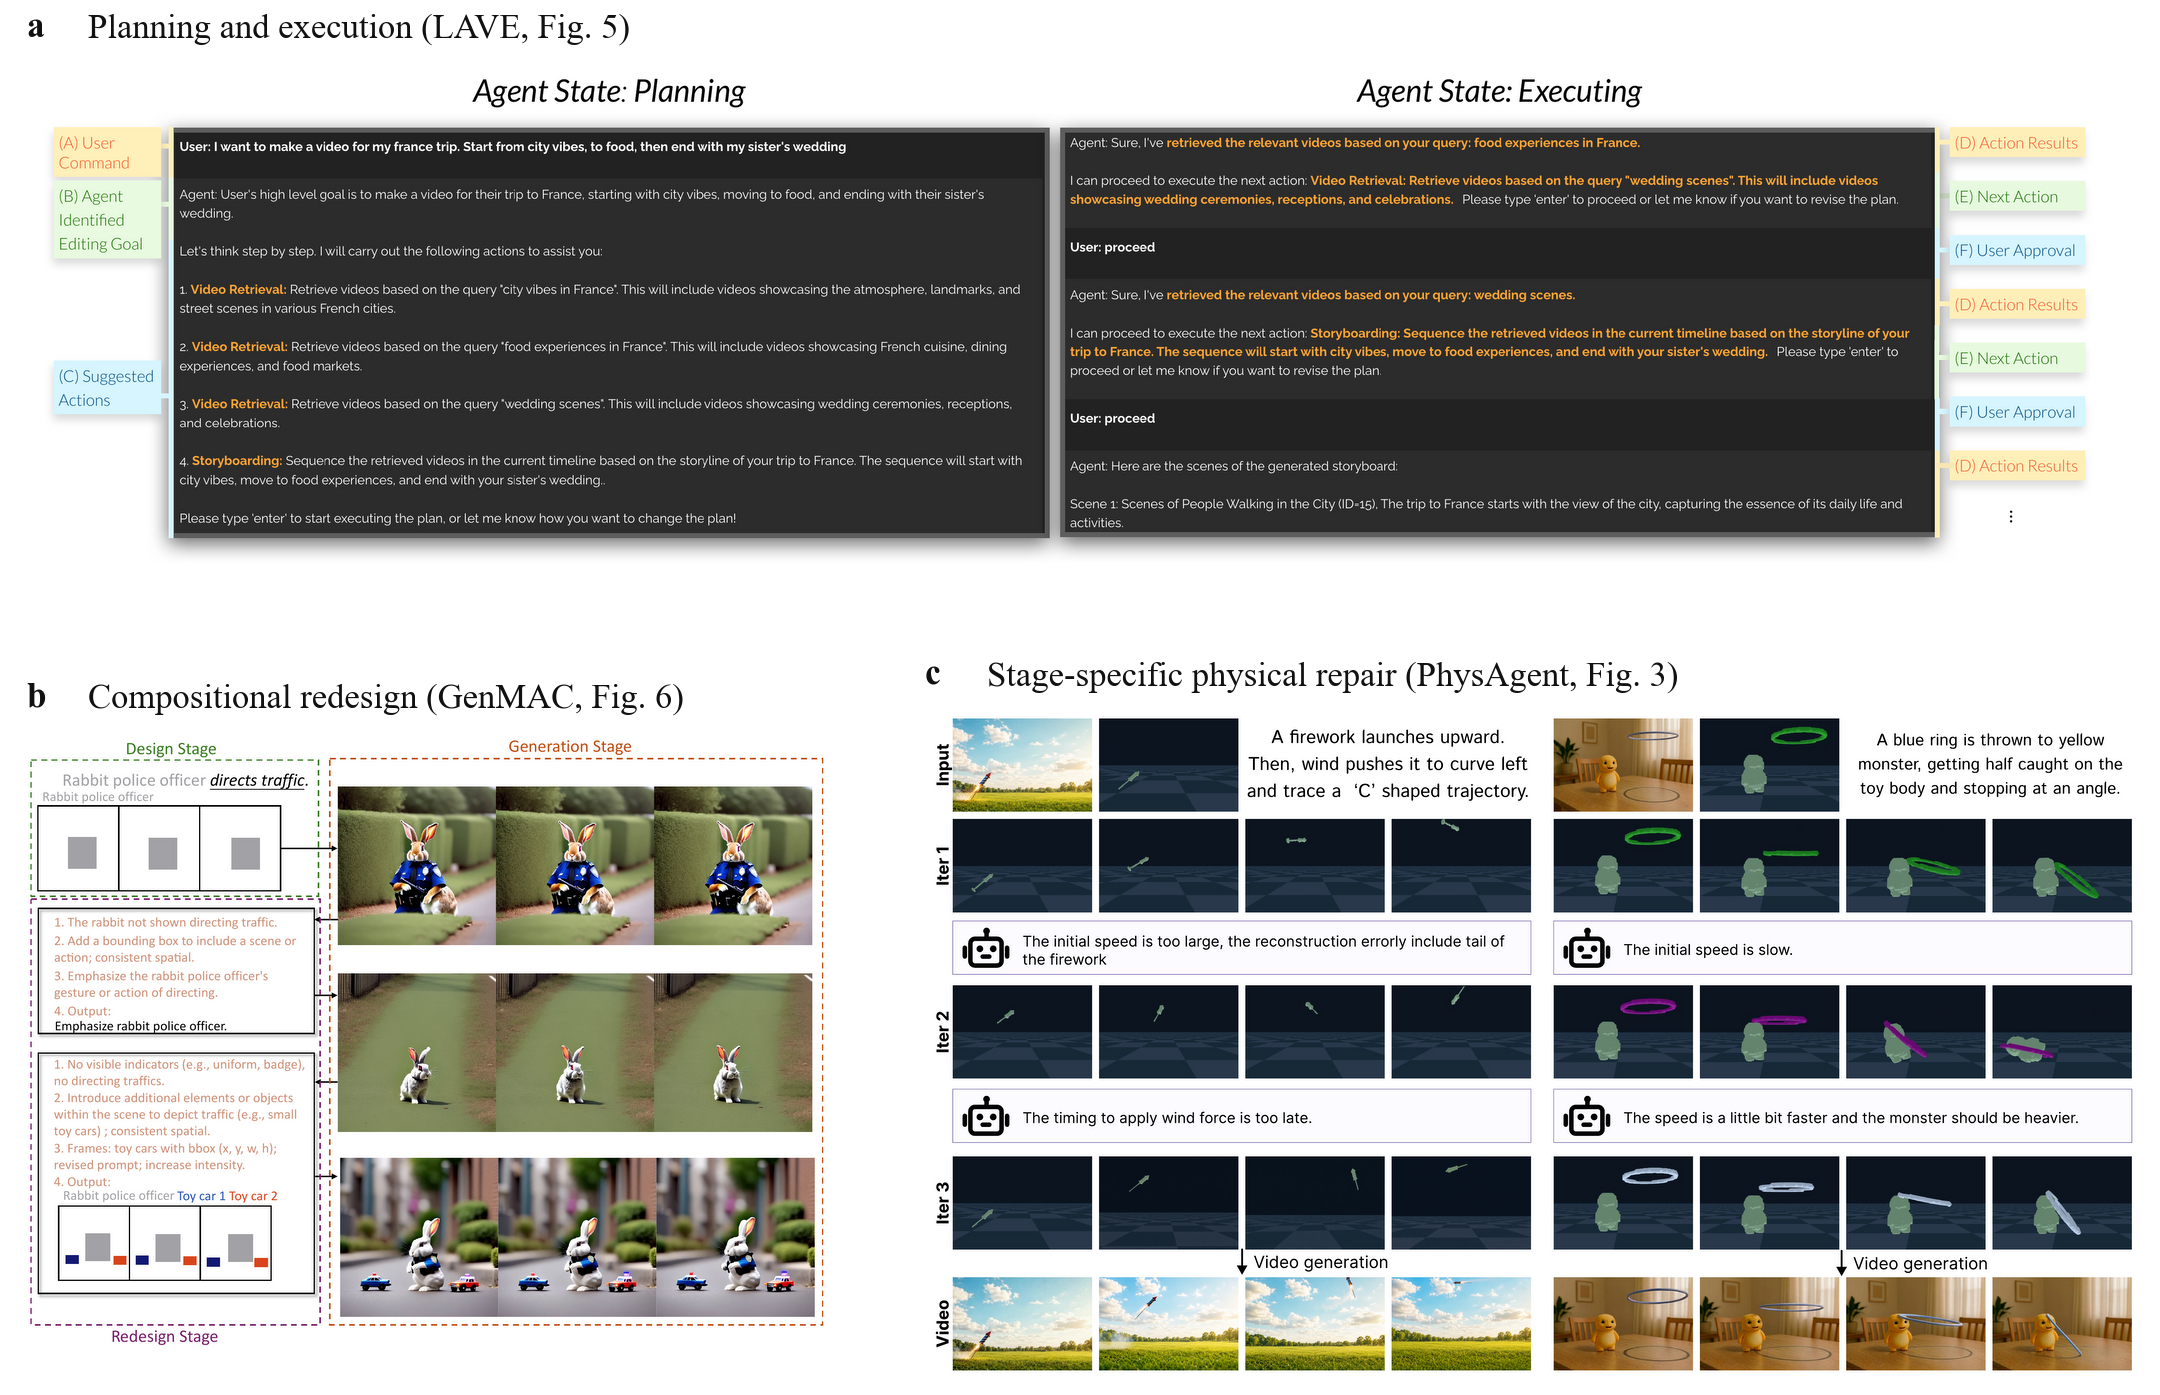
\includegraphics[width=\textwidth]{figures/ch5_artifact_conditioned_revision.jpg}
  \caption{Representative forms of artifact-conditioned revision. (a) LAVE separates planning from execution and retains user approval between the two states. (b) GenMAC revises compositional conditions through an iterative Design--Generation--Redesign loop. (c) PhysAgent uses stage-specific visual evidence to diagnose and repair physical programs before final video synthesis. Together, these examples show how intermediate observations can change later actions at the interface, generation, and simulation levels~\cite{wang2024lave,huang2024genmac,li2026physagent}.}
  \label{fig:ch5-artifact-revision}
\end{figure}

\paragraph{SCMAPR}
 performs self-correcting prompt refinement for complex text-to-video scenarios through stage-wise multi-agent collaboration. A Scenario Router assigns the request to a taxonomy-grounded scenario, a Policy Generator constructs a corresponding rewriting strategy, and a Prompt Refiner produces the revised prompt. Semantic verification then decomposes the original request into atomic elements and checks whether they are preserved in the refined prompt; detected omissions or contradictions trigger targeted revision before the prompt is passed to the video generator~\cite{avg260405489}.

\subsection{Skill evolution and diagnostic evidence.}
Two systems go beyond one-off correction by retaining what previous failures reveal. SCPE stores prompting lessons in a Playbook, whereas VideoWeaver refines reusable composition skills across long-video tasks.

\paragraph{SCPE}
 uses image-to-video generation as a diagnosable process for human--object interaction editing. An Analyzer inspects generated video frames to identify interaction failures, a Reflector abstracts these failures into reusable insights, and a Curator stores them in a Dynamic Playbook that links recurring failure patterns to prompting strategies. The updated Playbook guides subsequent prompt refinement, allowing experience from previous failures to transfer across editing samples, after which the best-aligned video frame is selected as the final edited image~\cite{avg260619073}.

\paragraph{VideoWeaver}
 studies how general-purpose agent harnesses can construct and improve workflows for long-video generation by composing multimodal foundation skills rather than following predefined pipelines. An agent-as-judge evaluates both execution traces and final videos, using evidence from metadata and intermediate artifacts to diagnose process and output failures. The resulting feedback drives a skill-evolution procedure that progressively refines composition and creator skills and merges them into reusable workflows that can improve performance on later and unseen tasks~\cite{avg260608091}. Figure~\ref{fig:ch5-state-experience} relates this cross-task skill evolution to within-trajectory state persistence.

\begin{figure}[p]
  \centering
  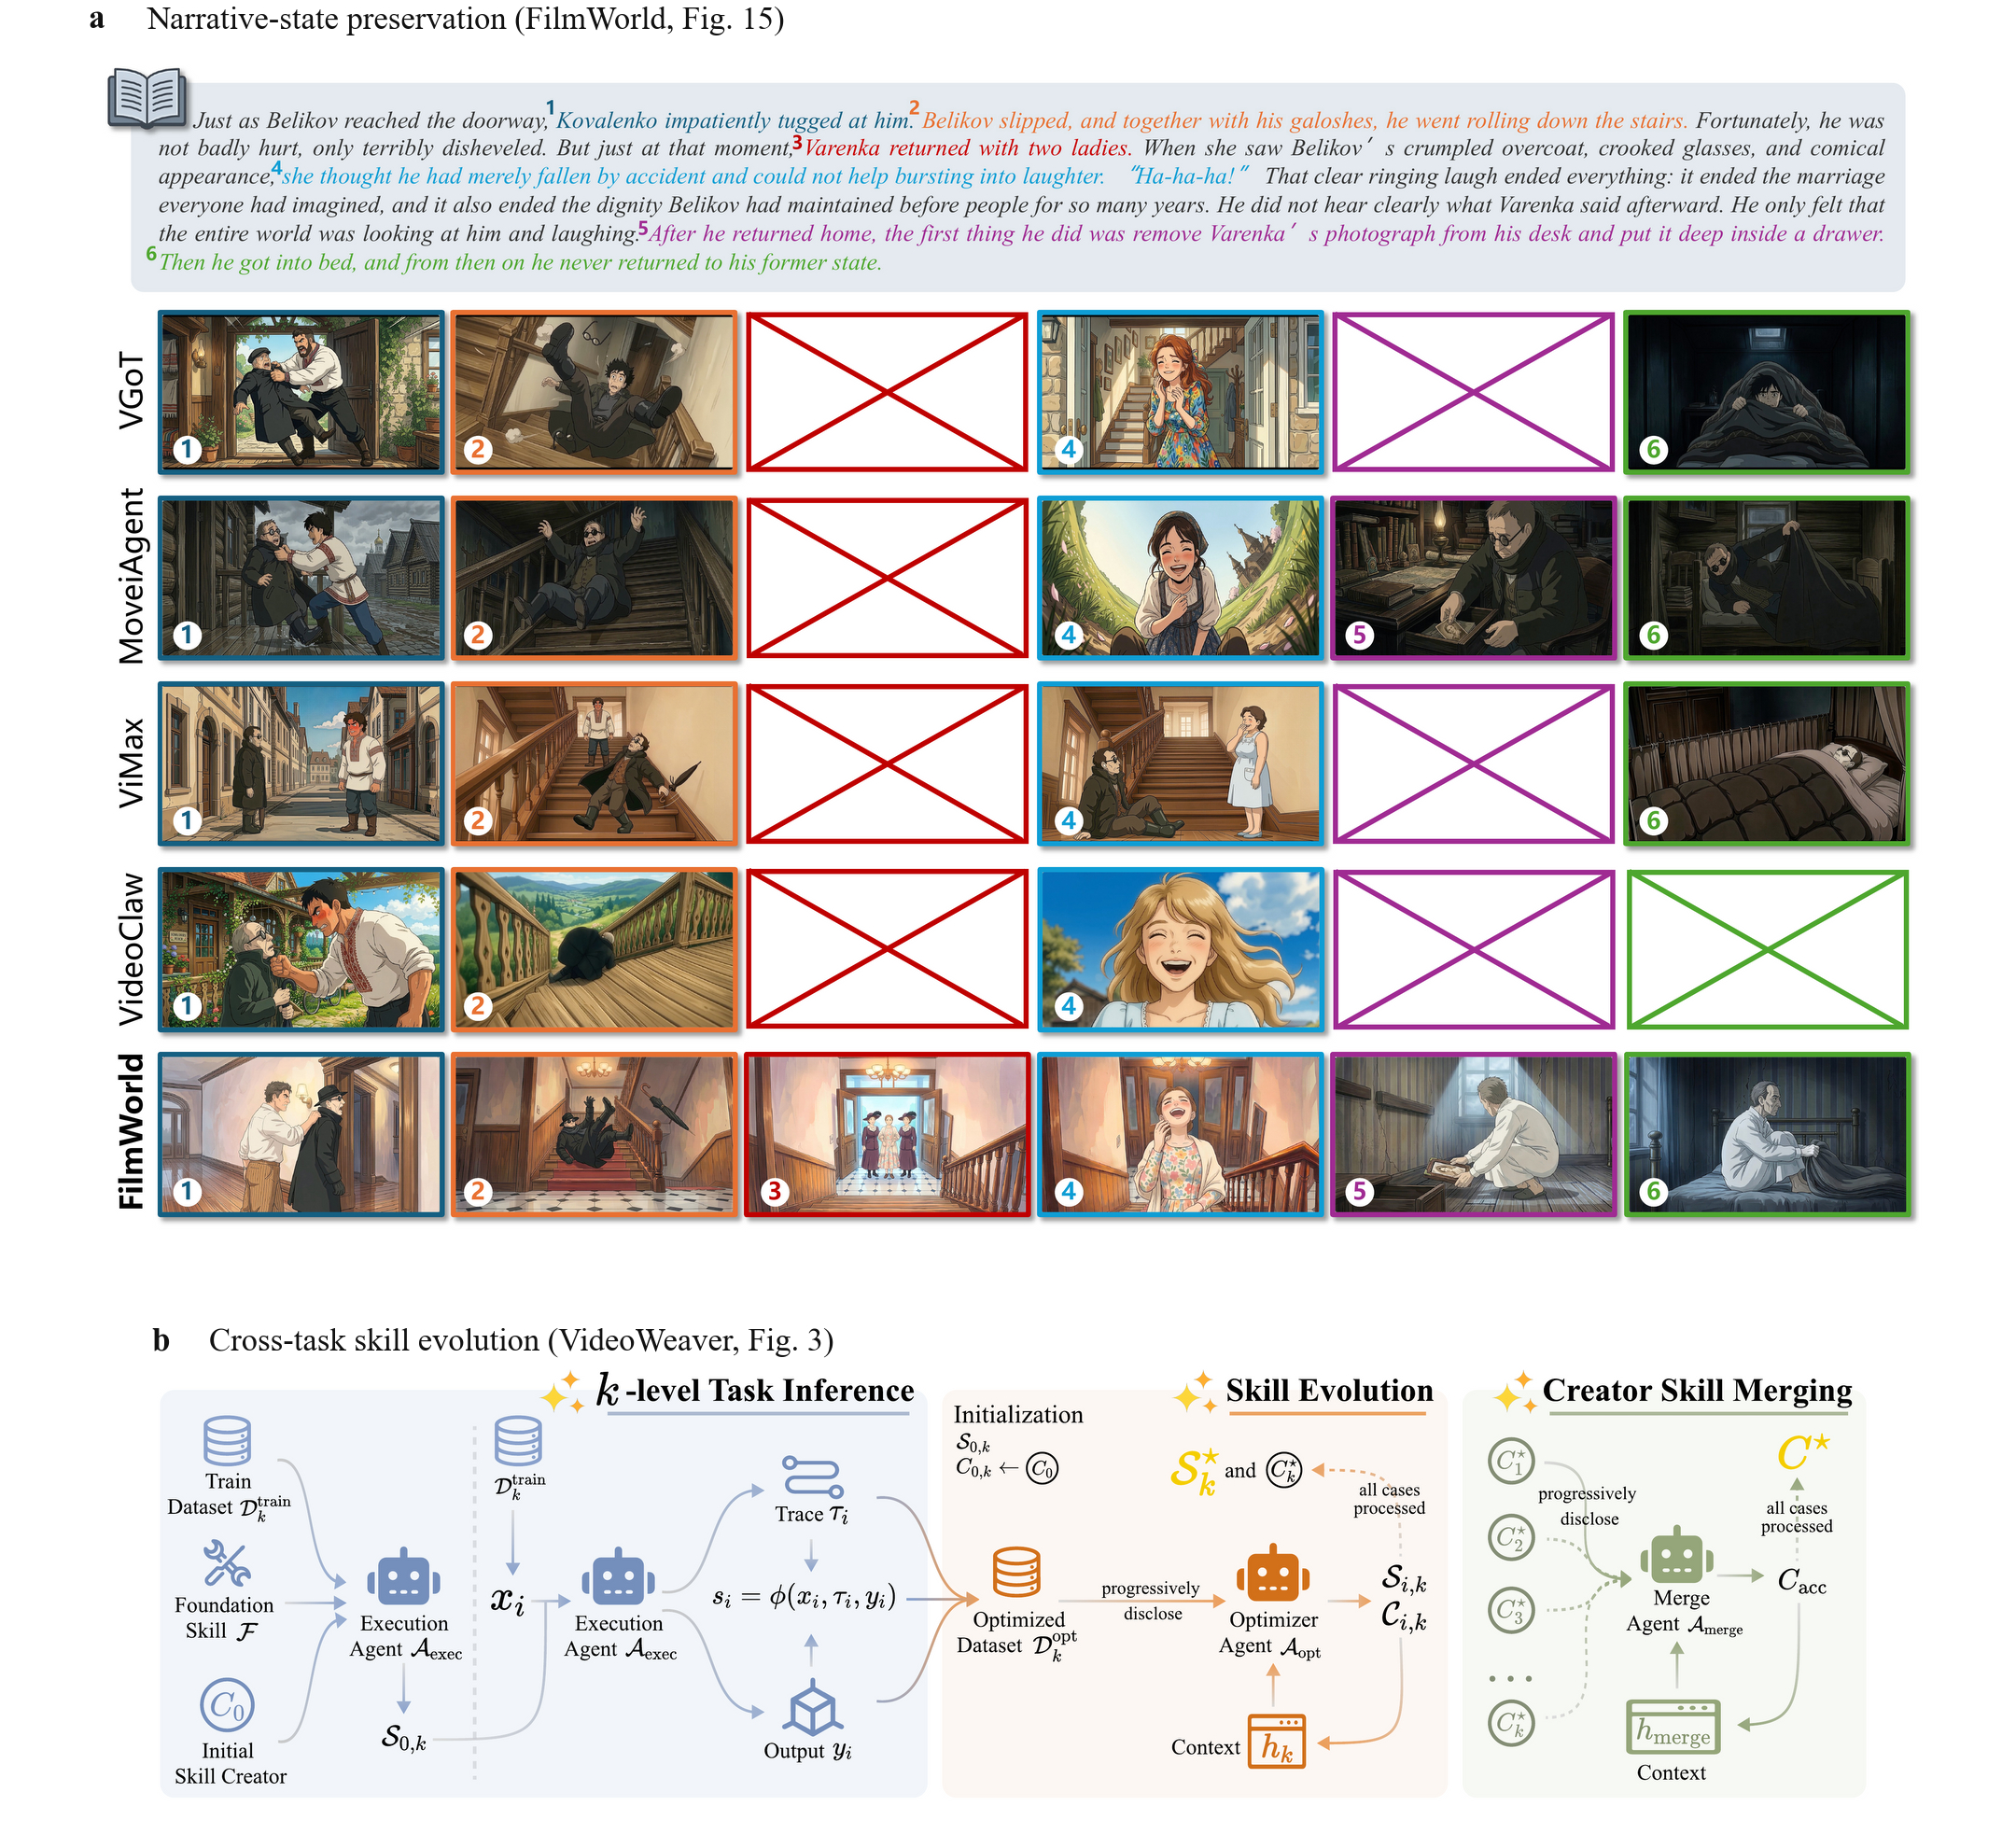
\includegraphics[width=\textwidth]{figures/ch5_state_experience_persistence.jpg}
  \caption{Persistence at two timescales. (a) FilmWorld compares narrative fidelity across six causally linked events, illustrating world-state maintenance within a long generation trajectory. (b) VideoWeaver transforms execution traces and evaluation feedback into evolved and merged skills for later tasks, illustrating cross-task experience reuse~\cite{avg260719038,avg260608091}.}
  \label{fig:ch5-state-experience}
\end{figure}

\begin{keytakeaway}[Key Takeaways]
Agentic video generation is progressing from structured production toward feedback-driven and experience-aware control. Stronger agents maintain state across a generation trajectory, repair localized failures, and convert diagnostic evidence into reusable prompting strategies or composition skills. Whether retained experience reliably improves future decisions under comparable time, compute, and tool budgets remains an open question.
\end{keytakeaway}

\FloatBarrier
